\usepackage{amsmath}
\usepackage{minted}
\usepackage{graphicx}
\graphicspath{ {.} }

\begin{enumerate}
\def\labelenumi{\arabic{enumi}.}
\item
  \begin{enumerate}  
  \def\labelenumii{\alph{enumii}.}
  \item
    \(p(X_2=Happy) = 0.9\)\\
  \item
    \(p(Y_2=Frown) = p(y_2=Frown|X_2=Happy)p(X_2=happy) + p(y_2=Frown|X_2=Sad)p(X_2=Sad)=0.1*0.9 + 0.6 * 0.1 = 0.15\)
  \item
    \(p(X_2=Happy | Y_2 = Frown) = \frac{p(X_2=happy)p(Y_2 = frown | X_2 = happy)}{p(Y_2 = frown)} = \frac{0.9 \cdot 0.1}{0.15} = 0.6\)
  \item

    Note that \[  
        \begin{pmatrix}
            p(X_j = Happy) \\
            p(X_j = Sad)
        \end{pmatrix}
        =
        \begin{pmatrix}
            0.9 & 0.1 \\
            0.1 & 0.9 
        \end{pmatrix}^{j - 1}
        \cdot
        \begin{pmatrix}
            1 \\
            0
        \end{pmatrix}
        \].

        Then \[
        \begin{pmatrix}
            p(X_{80} = Happy) \\
            p(X_{80} = Sad)
        \end{pmatrix}
        =
        \begin{pmatrix}
            0.9 & 0.1 \\
            0.1 & 0.9 
        \end{pmatrix}^{79}
        \cdot
        \begin{pmatrix}
            1 \\
            0
        \end{pmatrix}
        \approx
        \begin{pmatrix}
            0.5 && 0.5 \\
            0.5 && 0.5
        \end{pmatrix} 
        \cdot
        \begin{pmatrix}
            1 \\
            0
        \end{pmatrix}
        =
        \begin{pmatrix}
            0.5 \\
            0.5
        \end{pmatrix}
        \] So
    \(p(Y_{80}=yell) = p(y_{80}=yell|X_{80}=Happy)p(X_{80}=happy) + p(y_{80}=yell|X_{80}=Sad)p(X_{80}=Sad)\approx0.1*0.5 + 0.2 * 0.5 = 0.15\).
  \item
    Note that
    \begin{equation}
        \begin{split}
            & \mbox{argmax}_{x_1,\cdots,x_5} p(X_1=x_1,\cdots,X_5=x_5|Y_1=...=Y_5=frown) = \\
            & \mbox{argmax}_{x_1,\cdots,x_5} \frac
                {
                    p(X_1=x_1,\cdots,X_5=x_5)p(Y_1=...=Y_5=frown|X_1=x_1,\cdots,X_5=x_5)
                }
                {
                    p(Y_1=...=Y_5=frown)
                } = \\
            & \mbox{argmax}_{x_1,\cdots,x_5} p(X_1=x_1,\cdots,X_5=x_5)p(Y_1=...=Y_5=frown|X_1=x_1,\cdots,X_5=x_5)
        \end{split}
    \end{equation}
    Let $n_{happy}$ be the number of days where Harry is happy. We know that 
    \begin{equation}
        \begin{split}
        p(Y_1=...=Y_5=frown|X_1=x_1,\cdots,X_5=x_5) & = \prod_{i=1}^5 p(Y_i=frown | X_i=x_i) \\
        & = 0.1 ^ {n_{happy}} * 0.2 ^ {(5 - n_{happy})}
        \end{split}
    \end{equation}
    and that for $p(X_1=x_1,\cdots X_5=x_5|n_{happy})$ to be maximized there should be at most one transition between states such that  
        \begin{equation}
            x_i = 
                \begin{cases}
                    Happy, & \text{if } i \leq n_{happy} \\
                    Sad, & \text{otherwise.}
                \end{cases}
        \end{equation}
    Hence, 
        \begin{equation}
            \mbox{max}_{x_1,\cdots,x_5} p(X_1=x_1,\cdots X_5=x_5|n_{happy}) = 
                \begin{cases}
                    0.9^5 & \mbox{if } n_{happy} = 5 \\
                    0.9^4 * 0.1 & \mbox{otherwise}
                \end{cases}
        \end{equation}
    Solving analytically we can see that
    \begin{equation}
    	\mbox{argmax}_{n_{happy}} p(X_1=x_1,\cdots,X_5=x_5)p(Y_1=...=Y_5=frown|X_1=x_1,\cdots,X_5=x_5) = 1
    \end{equation}
    Therefore, $X_1 = happy$ and $X_2 = X_3 = X_4 = X_5 = sad$.
  \end{enumerate}
  \item Suppose we have a directed graph $G$ with two nodes $u$ and $v$, edges $u\to v$ and $v\to u$ and the random variables $X_u$ and $X_v$ each of which can take on the values $a$ and $b$. 

  Consider
    \begin{equation}
        f_u(x_u | x_{pa(u)}) = 
            \begin{cases}
                0 & \mbox{if } x_v \not= x_u \\
                1 & \mbox{if } x_v = x_u
            \end{cases}
    \end{equation}
  and 
    \begin{equation}
        f_v(x_v | x_{pa(v)}) = 
            \begin{cases}
                0 & \mbox{if } x_v = x_u \\
                1 & \mbox{if } x_v \not= x_u
            \end{cases}
    \end{equation}
  which specify distributions over $X_u$ and $X_v$ respectively. Further, note that for any given values of $x_u$ and $x_v$, $f(x_u, x_v) = f_u(x_u | x_v)f_v(x_v | x_u) = 0$. Hence, 
    \begin{equation}
        \sum_{x_u,x_v} f(x_u,x_v) = 0 \not = 1
    \end{equation}
  and thus does not a define a valid probability distribution.

\item
  \begin{enumerate}
  \def\labelenumii{\alph{enumii}.}
	  \item (1, 2), (1, 3), (1, 5), (1, 7), (1, 8), (1, 9), (1, 10), (2, 7), (2, 8), (3, 7), (3, 8), (4, 8), (6, 7), (6, 8), (7, 8), (7, 10), (8, 9), (8, 10)
	  \item $A = {3, 5, 7, 8, 10}$
  \end{enumerate}
\item First note that since 
  \begin{equation}
		Pr(x) = Pr(x, 0, 0) + Pr(x, 0, 1) + Pr(x, 1, 0) + Pr(x, 1, 1) = \frac{1}{2}
	\end{equation}
	\begin{equation}
		Pr(y) = Pr(0, y, 0) + Pr(0, y, 1) + Pr(1, y, 0) + Pr(1, y, 1) = \frac{1}{2}
	\end{equation}
\begin{equation}
	Pr(x, y) = Pr(x, y, 1) + Pr(x, y, 0) = \frac{1}{4}
\end{equation}
that $Pr(x, y) = Pr(x)Pr(y)$ and thus $X\perp Y \in I(Pr)$. We can show by the same argument that $X \perp Z, Y \perp Z \in I(Pr)$. 

Further note that since
\begin{equation}
	Pr(x, y | z) = 
		\frac{Pr(x, y, z)}{Pr(z)} = 
		\begin{cases}
			\frac{1}{6} & \mbox{if } x\oplus y = z \\
			\frac{1}{3}  & \mbox{otherwise}
		\end{cases}
  
\end{equation}
\begin{equation}
	Pr(x | z) = \frac{Pr(x, z)}{Pr(z)} = \frac{1}{2}
\end{equation}
\begin{equation}
	Pr(y | z) = \frac{Pr(y, z)}{Pr(z)} = \frac{1}{2}
\end{equation}
that $Pr(x, y | z) \not= Pr(x | z)Pr(y | z)$. By a similar argument, $X\perp Y | Z, X\perp Z |Y, Y \perp Z | X \not\in I(Pr)$.

Now suppose there exists a graph $G$ such that $I(Pr) = I(G)$. Choose $A, B \in V(G)$ and suppose that $A\to B \in E(G)$. Then there is an active path connecting $A$ and $B$ and thus $A \perp B\not\in I(G)$, a contradiction. So there can be no edges connecting nodes in $G$ and thus $G$ is a disconnected graph. If $G$ is a disconnected graph, then there are no trails connecting $X$ and $Y$. Thus, when $Z$ is activated there can be no active trails connecting $X$ and $Y$. Thus, by definition, $X$ are d-separated by $Z$ and thus $X\perp Y | Z \in I(G)$. But then $X \perp Y | Z \in I(Pr)$, a contradiction. Therefore, there does not exist a graph $G$ such that $I(Pr) = I(G)$.

\item
	Here is the library code I built to answer the questions in the prompt.

   \begin{minted}{python}
from collections import Counter

import funcy
import numpy as np
import pandas as pd
from sklearn.metrics import zero_one_loss, confusion_matrix


def parse_dataset(filename):
    dataset_file = open(filename)
    X = []
    y = [] 
    for line in dataset_file:
        tokens = line.split()
        is_spam = int(tokens[1] == "spam")
        word_counts = {}
        for token, count in funcy.partition(2, tokens[2:]):
            word_counts[token] = int(count)
        X.append(word_counts)
        y.append(is_spam)
    return X, y


def calculate_class_priors(y):
    return funcy.walk_values(lambda v: v / len(y), dict(Counter(y)))


def m_estimate(n_c, p, m, n):
    return (n_c + p * m) / (m + n)


def sum_word_vectors(v):
    return funcy.merge_with(sum, *v)


def calculate_m_estimates(X, y, alpha=1.0):
    total_counts = sum_word_vectors(X)
    vocabulary = total_counts.keys()
    m = len(vocabulary) * alpha
    p = 1 / len(vocabulary)
    n = sum(total_counts.values())

    grouped_counts = {
        k: sum_word_vectors(v)
        for k, v in funcy.group_values(zip(y, X)).items()
    }
    counts_as_series = {
        k: pd.Series(v).reindex(vocabulary, fill_value=0) 
        for k, v in grouped_counts.items()
    }
    likelihood_m_estimates = {
        k: m_estimate(v, p, m, n)
        for k, v in counts_as_series.items()
    }

    return likelihood_m_estimates


class Classifier:
    def __init__(self, alpha):
        self.alpha = alpha

    def train(self, X, y):
        likelihood = calculate_m_estimates(X, y, self.alpha)
        self.log_likelihood = funcy.walk_values(np.log, likelihood)
        self.log_class_priors = funcy.walk_values(np.log, calculate_class_priors(y))

    def _predict_class_posterior(self, x, y):
        x_series = pd.Series(x)

        return self.log_class_priors[y] + np.sum(self.log_likelihood[y] * x_series)

    def predict(self, x):        
        return max(self.log_class_priors.keys(),
                   key=lambda y: self._predict_class_posterior(x, y))

   \end{minted}

   There are three main parts: a parser, an interface class used to train the model and make predictions, and some helper functions that contain the mathematical logic used by the model. The parser reads in a text file in the format that was provided and outputs an X, y pair where X is the input data structured as a python dictionary bag of words representation and y is a binary variable that is 1 if the email is spam and 0 otherwise. The interface class takes data in this format for both training and making predictions. For computational reasons some of the dictionaries are converted to pandas series at different points in the pipeline. 

   The training phase of the model takes the input X and y data and computes $\log(p(w|c))$ and $\log(p(c))$ for every word $w$ and class $c$. The model takes in an $\alpha$ parameter which is used to multiply the $m$ parameter in question $e$. The prediction step takes in a sample $x$ and calculates
   \begin{equation}
   	\mbox{argmax}_c \log(p(c)) + \sum_i x_{w_i}\log(p(w_i | c)) 
   \end{equation} 
   where $x_{w_i}$ is the number of times that $w_i$ appeared in sample $x$. This value is equivalent to the class argument that the maximizes the posterior probability.

   \begin{enumerate}
  	\setcounter{enumii}{1}
  	\def\labelenumii{\alph{enumii}.}
  	\item 
  	\begin{minted}{python}
	  	X_train, y_train = parse_dataset("train")

		# Spam percentage
		print("P(spam) = {}".format(sum(y_train) / len(y_train)))
	\end{minted}

  	$P(spam) = 0.57$
  	\item
  	\begin{minted}{python}
		# Most frequent words
		m_estimates = calculate_m_estimates(X_train, y_train)
		print("Top 5 ham words")
		print(m_estimates[0].sort_values(ascending=False).head())
		print("Top 5 spam words")
		print(m_estimates[1].sort_values(ascending=False).head())
	\end{minted}

  		The 5 most likely words given that the document is spam are ``enron'', ``a'', ``corp'', ``the'' and ``to''. The 5 most likely words given that a document is ham are `aaaaaaaaaaaaaaaaaaaaaaaaaaaaaaaaaaaaaaaaaaaaaaaaaaaaaaaaaaaaaaaaaaaaaaaaaaaa', `enron', `the', `to' and `a'.
  	\item 
  	\begin{minted}{python}
	    classifier = Classifier(alpha)
	    classifier.train(X_train, y_train)

	    y_predicted = [classifier.predict(x) for x in X_test]
	    print("Loss for alpha {} is {}".format(alpha, zero_one_loss(y_test, y_predicted)))
	test_alpha(1)
	\end{minted}

  	The accuracy is 0.086.
  	\item 

  	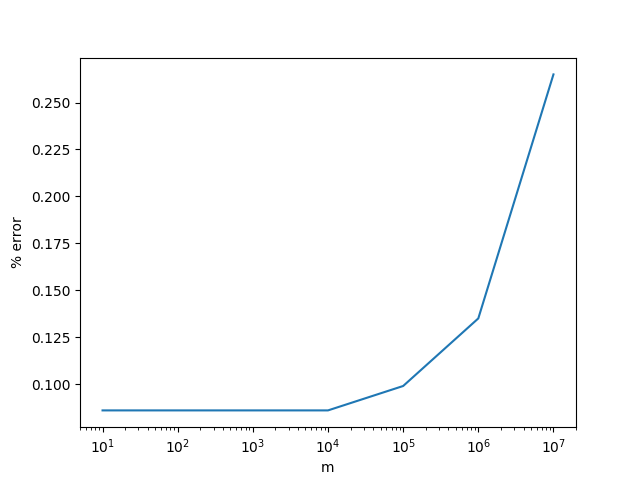
\includegraphics{error_plot.png}

  	When $m$ is very large we are assuming that our training set is not very representative of our test set. When $m$ is very small we are assuming that the training set and test set are similar. Test accuracy is higher when we assuming that the training set and test set are very similar.

  	\item If I had access to the classifier, I would calculate $P(spam|w)$ and $P(ham|w)$ for all of the words and then remove words where $P(spam|w)$ was calculated to be much greater than $P(ham|w)$ and add words where the opposite was true.

  \end{enumerate}
\end{enumerate}